\documentclass[a4paper,10pt]{article}
\title{}
\author{}
\usepackage{graphicx} 

\begin{document}
\maketitle
\begin{abstract}

We consider the single parametered family of triangles in the hyperbolic two dimensional space that have two angles of size zero and one non zero angle.
More specifically we are interested in the Fangano triangles formed by connecting the bases of the (hyperbolic) heights of the triangles as shown in Figure 1, modeled as will be the whole document 
in the upper half plane model:

\begin{center}
 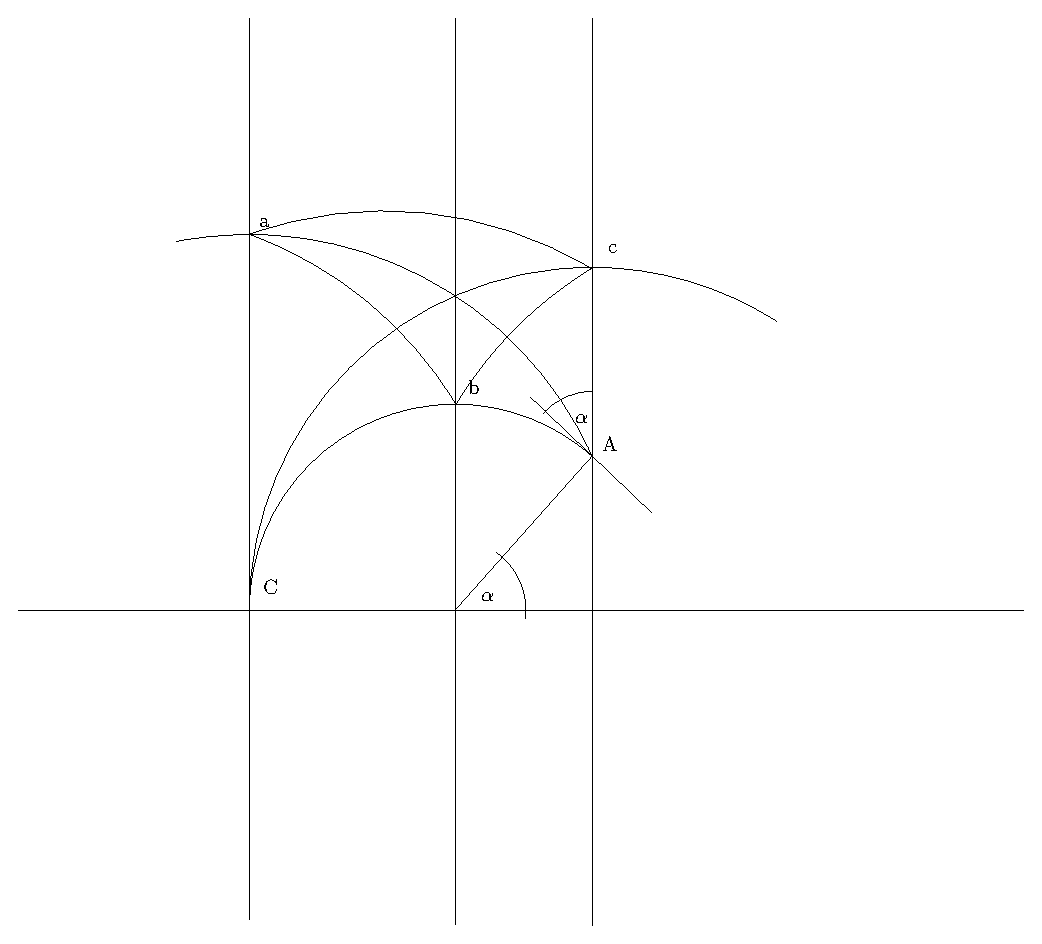
\includegraphics[width=12cm]{./hyper00a.eps}
 % hyper00a.eps: 0x0 pixel, 300dpi, 0.00x0.00 cm, bb=41 259 525 696
 Figure 1
\end{center}

Our goal is to understand what $\alpha$ maximizes the perimiter of such triangles 
and we will do so using simple calculus, we will develop the formula for the perimiter
of such triangles (based on $\alpha$), differentiate to find cirtical points and check
the value at the edges $\alpha = 0$ and $\alpha = \frac{\pi}{2}$

\end{abstract}
\section{}

Let us first find $a$, $b$ and $c$, the bases of the heights.

Since $B$ is located at $\infty$, it is trivial to see that

$b = 1 + \mathbf{\imath}$

Now, based on the fact that the edges leaving $A$ and $C$ towards $B$ (loacted at $\infty$) are perpendicular to the real axis
thus every hyperbolic line perpendicular to it is in fact an euclidean circle whose center is located on the real part of $A$ and $C$ respectfully. 
Knowing a line on the perpendicular and the center of the circle it runs along makes it easy to determine its radius which in tuen means that given
A point, it is easy to determine the base of the perpendicular leaving it - simply calculate its distance from $A$ or $C$ and that will be the imaginary
part of the base (the real part being the real part of $A$ or $C$ respectfully):

$a = \mathbf{\imath} \sqrt{2 + 2 cos\left(\alpha\right)}$

$c = \left(1 + \mathbf{\imath}\right) \left(1 + cos\left(\alpha\right)\right)$


Now let us calculate the hyperbolic distances between $a$, $b$ and $c$ using the formula:

$d\left(x,y\right) = acosh(\frac{\|x-y\|^{2}}{\Im\left(x\right)\Im\left(y\right)})$

$d\left(a, b\right) =$
$acosh\left(1 + \frac{\left(\Im\left(a - b\right)\right)^{2} + \left(\Re\left(a - b\right)\right)^{2}}{2 \sqrt{2 + 2 cos\left(\alpha\right)}}\right) =$
$acosh\left(1 + \frac{1 + \left(1 - \sqrt{2 + 2 cos\left(\alpha\right)}\right)^{2}}{2 \sqrt{2 + 2 cos\left(\alpha\right)}}\right) =$
$acosh\left(1 + \frac{4 + 2 cos\left(\alpha\right) - 2 \sqrt{2 + 2 cos\left(\alpha\right)}}{2 \sqrt{2 + 2 cos\left(\alpha\right)}}\right) =$
$acosh\left(\frac{4 + 2 cos\left(\alpha\right)}{2 \sqrt{2 + 2 cos\left(\alpha\right)}}\right) =$
$acosh\left(\frac{2 + cos\left(\alpha\right)}{\sqrt{2 + 2 cos\left(\alpha\right)}}\right) =$


$d\left(b, c\right) = $
$acosh\left(1 + \frac{\left(\Im\left(b - c\right)\right)^{2} + \left(\Re\left(b - c\right)\right)^{2}}{2 + 2 cos\left(\alpha\right)}\right) =$
$acosh\left(1 + 2 \frac{cos^{2}\left(\alpha\right)}{2 + 2 cos\left(\alpha\right)}\right) =$
$acosh\left(1 + \frac{cos^{2}\left(\alpha\right)}{1 + cos\left(\alpha\right)}\right) =$
$acosh\left(\frac{1 + cos\left(\alpha\right) + cos^{2}\left(\alpha\right)}{1 + cos\left(\alpha\right)}\right) =$


$ d\left(c, a\right)=$
$acosh\left(1 + \frac{\left(\Im\left(c - a\right)\right)^{2} + \left(\Re\left(c - a\right)\right)^{2}}{\left(2 + 2 cos\left(\alpha\right)\right)^{\frac{3}{2}}}\right) =$
$acosh\left(1 + \frac{\left(1 + cos\left(\alpha\right)\right)^{2} + \left(1 + cos\left(\alpha\right) - \sqrt{2 + 2 cos\left(\alpha\right)}\right)^{2}}{\left(2 + 2 cos\left(\alpha\right)\right)^{\frac{3}{2}}}\right) =$
$acosh\left(1 + \frac{3 + 4 cos\left(\alpha\right) + \left(1 + cos\left(\alpha\right)\right)^{2} + cos^{2}\left(\alpha\right) - \left(2 + 2 cos\left(\alpha\right)\right)^{\frac{3}{2}}}{\left(2 + 2 cos\left(\alpha\right)\right)^{\frac{3}{2}}}\right) =$
$acosh\left(1 + \frac{4 + 6 cos\left(\alpha\right) + 2 cos^{2}\left(\alpha\right) - \left(2 + 2 cos\left(\alpha\right)\right)^{1.5}}{\left(2 + 2 cos\left(\alpha\right)\right)^{\frac{3}{2}}}\right) =$
$acosh\left(1 + \frac{4 + 6 cos\left(\alpha\right) + 2 cos^{2}\left(\alpha\right) - \left(2 + 2 cos\left(\alpha\right)\right)^{1.5}}{\left(2 + 2 cos\left(\alpha\right)\right)^{\frac{3}{2}}}\right) =$
$acosh\left(1 + \frac{4 + 6 cos\left(\alpha\right) + 2 cos^{2}\left(\alpha\right) - \left(2 + 2 cos\left(\alpha\right)\right)^{1.5}}{\left(2 + 2 cos\left(\alpha\right)\right)^{1.5}}\right) =$
$acosh\left(\frac{4 + 6 cos\left(\alpha\right) + 2 cos^{2}\left(\alpha\right)}{\left(2 + 2 cos\left(\alpha\right)\right)^{1.5}}\right) =$
$acosh\left(\frac{\sqrt{2} \left(2 + 3 cos\left(\alpha\right) + cos^{2}\left(\alpha\right)\right)}{\left(1 + cos\left(\alpha\right)\right)^{1.5}}\right) =$
$acosh\left(\frac{\sqrt{2} \left(2 + 3 cos\left(\alpha\right) + cos^{2}\left(\alpha\right)\right)}{2 \left(1 + cos\left(\alpha\right)\right)^{1.5}}\right) =$
$acosh\left(\frac{2 + cos\left(\alpha\right)}{\sqrt{2 + 2 cos\left(\alpha\right)}}\right) =$
$ d\left(a, b\right) $


And differentiate (with respect to $\alpha$):


$\frac{d}{d\alpha}d\left(b,c\right)=$

$\frac{- \frac{sin\left(\alpha\right)}{\left(2 + 2 cos\left(\alpha\right)\right)^{0.5}} + 2 \frac{\left(1.0 + 0.5 cos\left(\alpha\right)\right) sin\left(\alpha\right)}{\left(2 + 2 cos\left(\alpha\right)\right)^{1.5}}}{\left(-1 + \frac{\left(2 + cos\left(\alpha\right)\right)^{2}}{2 + 2 cos\left(\alpha\right)}\right)^{0.5}}=$
$\sqrt{\frac{2 + 2 cos\left(\alpha\right)}{2 + 2 cos\left(\alpha\right) + cos^{2}\left(\alpha\right)}} \left(- \frac{sin\left(\alpha\right)}{\left(2 + 2 cos\left(\alpha\right)\right)^{0.5}} + 2 \frac{\left(1.0 + 0.5 cos\left(\alpha\right)\right) sin\left(\alpha\right)}{\left(2 + 2 cos\left(\alpha\right)\right)^{1.5}}\right)=$
$- \frac{\sqrt{\frac{2 + 2 cos\left(\alpha\right)}{2 + 2 cos\left(\alpha\right) + cos^{2}\left(\alpha\right)}} \left(1 - \frac{2 + cos\left(\alpha\right)}{2 + 2 cos\left(\alpha\right)}\right) sin\left(\alpha\right)}{\sqrt{2 + 2 cos\left(\alpha\right)}}=$
$- \frac{\sqrt{\frac{2 + 2 cos\left(\alpha\right)}{2 + 2 cos\left(\alpha\right) + cos^{2}\left(\alpha\right)}} cos\left(\alpha\right) sin\left(\alpha\right)}{\left(2 + 2 cos\left(\alpha\right)\right)^{\frac{3}{2}}}=$
$- \sqrt{\frac{1}{\left(2 + 2 cos\left(\alpha\right)\right)^{2} \left(2 + 2 cos\left(\alpha\right) + cos^{2}\left(\alpha\right)\right)}} cos\left(\alpha\right) sin\left(\alpha\right)=$
$- \frac{cos\left(\alpha\right) sin\left(\alpha\right)}{\sqrt{2 + 2 cos\left(\alpha\right) + cos^{2}\left(\alpha\right)} \left(2 + 2 cos\left(\alpha\right)\right)}$


$\frac{d}{d\alpha}d\left(a, b\right)=\frac{d}{d\alpha}d\left(c, a\right)=$

$\frac{cos^{2}\left(\alpha\right) sin\left(\alpha\right) - 2 \left(1 + cos\left(\alpha\right)\right) cos\left(\alpha\right) sin\left(\alpha\right)}{\left(1 + cos\left(\alpha\right)\right)^{2} \left(-1 + \frac{\left(1 + cos\left(\alpha\right) + cos^{2}\left(\alpha\right)\right)^{2}}{\left(1 + cos\left(\alpha\right)\right)^{2}}\right)^{0.5}}=$
$\frac{cos^{2}\left(\alpha\right) sin\left(\alpha\right) - 2 \left(1 + cos\left(\alpha\right)\right) cos\left(\alpha\right) sin\left(\alpha\right)}{\left(1 + cos\left(\alpha\right)\right)^{2} \left(-1 + \left(1 + \frac{cos^{2}\left(\alpha\right)}{1 + cos\left(\alpha\right)}\right)^{2}\right)^{0.5}}=$
$\frac{cos^{2}\left(\alpha\right) sin\left(\alpha\right) - 2 \left(1 + cos\left(\alpha\right)\right) cos\left(\alpha\right) sin\left(\alpha\right)}{\left(1 + cos\left(\alpha\right)\right)^{2} \left(2 \frac{cos^{2}\left(\alpha\right)}{1 + cos\left(\alpha\right)} + \frac{cos^{4}\left(\alpha\right)}{\left(1 + cos\left(\alpha\right)\right)^{2}}\right)^{0.5}}=$
$\frac{cos^{2}\left(\alpha\right) sin\left(\alpha\right) - 2 \left(1 + cos\left(\alpha\right)\right) cos\left(\alpha\right) sin\left(\alpha\right)}{\left(\frac{2 + 2 cos\left(\alpha\right) + cos^{2}\left(\alpha\right)}{\left(1 + cos\left(\alpha\right)\right)^{2}}\right)^{0.5} \left(1 + cos\left(\alpha\right)\right)^{2} cos\left(\alpha\right)}=$
$\frac{cos^{2}\left(\alpha\right) sin\left(\alpha\right) - 2 \left(1 + cos\left(\alpha\right)\right) cos\left(\alpha\right) sin\left(\alpha\right)}{\sqrt{2 + 2 cos\left(\alpha\right) + cos^{2}\left(\alpha\right)} \left(1 + cos\left(\alpha\right)\right) cos\left(\alpha\right)}=$
$\frac{cos^{2}\left(\alpha\right) sin\left(\alpha\right) - 2 \left(1 + cos\left(\alpha\right)\right) cos\left(\alpha\right) sin\left(\alpha\right)}{\sqrt{2 + 2 cos\left(\alpha\right) + cos^{2}\left(\alpha\right)} \left(1 + cos\left(\alpha\right)\right) cos\left(\alpha\right)}=$
$\frac{\left(- \left(2 + 2 cos\left(\alpha\right)\right) cos\left(\alpha\right) + cos^{2}\left(\alpha\right)\right) sin\left(\alpha\right)}{\sqrt{2 + 2 cos\left(\alpha\right) + cos^{2}\left(\alpha\right)} \left(1 + cos\left(\alpha\right)\right) cos\left(\alpha\right)}=$
$- \frac{\left(2 + cos\left(\alpha\right)\right) sin\left(\alpha\right)}{\sqrt{2 + 2 cos\left(\alpha\right) + cos^{2}\left(\alpha\right)} \left(1 + cos\left(\alpha\right)\right)}$



$\frac{d}{d\alpha}\left(d\left(a, b\right) + d\left(b, c\right) + d\left(c, a\right)\right) = $
$\frac{d}{d\alpha}\left(2d\left(a, b\right) + d\left(b, c\right)\right) = $


$- \frac{\left(2 + cos\left(\alpha\right)\right) sin\left(\alpha\right)}{\sqrt{2 + 2 cos\left(\alpha\right) + cos^{2}\left(\alpha\right)} \left(1 + cos\left(\alpha\right)\right)} - 2 \frac{cos\left(\alpha\right) sin\left(\alpha\right)}{\sqrt{2 + 2 cos\left(\alpha\right) + cos^{2}\left(\alpha\right)} \left(2 + 2 cos\left(\alpha\right)\right)} =$
$\frac{- \left(2 + cos\left(\alpha\right)\right) sin\left(\alpha\right) - cos\left(\alpha\right) sin\left(\alpha\right)}{\sqrt{2 + 2 cos\left(\alpha\right) + cos^{2}\left(\alpha\right)} \left(1 + cos\left(\alpha\right)\right)} $
$- 2 \frac{sin\left(\alpha\right)}{\sqrt{2 + 2 cos\left(\alpha\right) + cos^{2}\left(\alpha\right)}} =$
$- 2 \frac{sin\left(\alpha\right)}{\sqrt{2 + 2 cos\left(\alpha\right) + cos^{2}\left(\alpha\right)}} =$
\end{document}
